\documentclass[10pt,a4j]{jarticle}
\newcommand{\setcounters}[1] {
  \setcounter{equation}{#1}
  \setcounter{figure}{#1}
  \setcounter{table}{#1}
}

\newcommand{\unit}[1] {
  \hspace{1mm}\mathrm{[#1]}
}

\newcommand{\degc} {
  \hspace{1mm}\mathrm{[}{}^\circ\mathrm{C]}
}

\newcommand{\refig}[1]{図\ref{fig::#1}}
\newcommand{\refeq}[1]{式(\ref{eq::#1})}
\newcommand{\reftab}[1]{表\ref{tab::#1}}

\newcommand{\fig}[5] {
  \begin{figure}[#1]
    \begin{center}
      \includegraphics[width=#2\hsize]{#3}
    \end{center}
    \caption{#4}
    \label{fig::#5}
  \end{figure}
}

\makeatletter
\def\eq{\@ifstar\@eq\@@eq}
\def\@eq#1{\begin{equation*}#1\end{equation*}}
\def\@@eq#1#2{\begin{equation}#2\label{eq::#1}\end{equation}}
\makeatother

\newcommand{\diff}[2] {
  \frac{\mathrm{d}#1}{\mathrm{d}#2}
}

\newcommand{\pdiff}[2] {
  \frac{\partial #1}{\partial #2}
}


\newcommand{\ddt}[2][1] {
  \ifnum #1 < 2
    \frac{\mathrm{d}#2}{\mathrm{d}t}
  \else
    \frac{\mathrm{d}^#1#2}{\mathrm{d}t^#1}
  \fi
}

\newcommand{\e}[1] {
  \mathrm{e}^{#1}
}

\newcommand{\lparen}{(}
\catcode `( = \active
\newcommand{(}{\ifmmode\left\lparen\else\lparen\fi}

\newcommand{\rparen}{)}
\catcode `) = \active
\newcommand{)}{\ifmmode\right\rparen\else\rparen\fi}

\newcommand{\bmat}[1] {
  \begin{bmatrix} #1 \end{bmatrix}
}

% -- Package ---------------------------------------------------
\usepackage[dvipdfmx]{graphicx}
\usepackage{amsmath, amssymb}
\usepackage{bm}
\usepackage{fancyhdr}
\usepackage{here}
\usepackage{listings}
\usepackage{multirow}


% -- Margin Config ---------------------------------------------
\setlength{\textheight}{\paperheight}
\setlength{\topmargin}{4.6truemm} % 30mm(=1.0in+4.6mm)
\addtolength{\topmargin}{-\headheight}
\addtolength{\topmargin}{-\headsep}
\addtolength{\textheight}{-60truemm}

\setlength{\textwidth}{\paperwidth}
\setlength{\oddsidemargin}{-0.4truemm} % 25mm(=1.0in-0.4mm)
\setlength{\evensidemargin}{-0.4truemm}
\addtolength{\textwidth}{-50truemm}


% -- Renewcommand ----------------------------------------------
\renewcommand{\theequation}{\arabic{section}.\arabic{equation}}
\renewcommand{\thefigure}{\thesection.\arabic{figure}}
\renewcommand{\thetable}{\thesection.\arabic{table}}
\renewcommand{\lstlistingname}{ソースコード}
\renewcommand{\headrulewidth}{0mm} % fancy
\renewcommand{\labelenumi}{(\arabic{enumi})}


% -- Config for fancy package ----------------------------------
\pagestyle{fancy}
\rhead{\thepage}
\lhead{}
\cfoot{}


% -- Config for package listings -------------------------------
\lstset{
  basicstyle={\ttfamily \small},
  breaklines=true,
  frame=trBL,
  numbers=left,
  numberstyle={\ttfamily \small},
}



\begin{document}
\def\maintitle{知能制御PBL\\}
\def\subtitle{最終報告書(個人レポート)\\}
\def\affiliation{九州工業大学 工学部 機械知能工学科\\知能制御工学コース 西田健研究室\\}

\def\dates{
  \hspace{0mm} 提出日:2017年08月08日 \\
}

\def\members{
      報告者:{\large 14104131} \hspace{1mm} 山崎 達也   \\
  共同実験者:{\large 13104042} \hspace{1mm} 烏谷 崇大   \\
              {\large 14104043} \hspace{1mm} 桑野 僚大   \\
              {\large 14104034} \hspace{1mm} 下松八重 宏太 \\
              {\large 14104090} \hspace{1mm} 中尾 真人   \\
              {\large 14104111} \hspace{1mm} 本田 空    \\
              {\large 16104313} \hspace{1mm} 山下 翔    \\
}

\begin{titlepage}
  \vspace*{25mm}
  \begin{center}
    {\huge \maintitle} \vspace{5mm}
    {\Huge \subtitle}  \vspace{20mm}
    {\Large \dates}
  \end{center}
  \vspace{25mm}
  \begin{flushright}
    {\LARGE \affiliation}
    \vspace{10mm}
    {\Large \members}
  \end{flushright}
\end{titlepage}



\newpage
\section{目的}
学部3年までに学習した制御理論や電気回路,
情報工学の知識を使って, 競技場内を自律的に走行するロボットカーの製作を行う.
各研究室でチーム一丸となってプロジェクトを進行し,
共同で課題を達成することの難しさや楽しさを学び,
エンジニアとして仕事を進めるための素養を身に付ける.
情報工学の知識を使って, 競技場内を自律的に走行するロボットカーの製作を行う.
各研究室でチーム一丸となってプロジェクトを進行し,
共同で課題を達成することの難しさや楽しさを学び,


\section{Robot Car Race(RCR)2017競技ルール}
\subsection{ルール概要}
競技場には黄色のポールや,火災に見立てた複数の赤色のポールが設置されている.
ポールに接触せず,できるだけ速やかに火災を鎮火させる
消防ロボットカー(ロボカー)を作成する.

\subsection{競技場詳細}
競技場の全体図を図\ref{course}に示し,以下に詳細を説明する.
\begin{enumerate}
  \item 競技場は板張りの床であり,縦・横ともに $5400\unit{mm}$である.

  \item 競技場には黄色の固定ポールと赤色の火災ポールが設置されており,
        スタートからゴールまで,固定ポールには接触,
        火災ポールには衝突することなく通過しなければならない.

  \item 火災ポールは青色の鎮火ポールに赤色の幕を被せたものであり,
        上部におもりなどを落としたり,幕を剥がしたりすることで,
        鎮火ポールに変化させる(このポールの製作も行うこと).

  \item スタート後は右手に固定ポールを見ながら直進し,
        消火活動開始区間まで移動しなければならない.消火活動開始区間に
        進入後は,右折し,火災ポールを発見し次第,消火にあたる.

  \item すべての火災ポールを消火して,鎮火ポールに変化させたのち,
        ゴール地点で停止する.

  \item 火災ポールの配置は競技ごとに異なる.
        また,鎮火ポールが存在することもある.

  \item ポールは直径 $80\unit{mm}$・高さ $120\unit{mm}$の中空パイプであり,
        黄・赤・青の色が付けられている.
\end{enumerate}

\begin{figure}[t]
  \begin{center}
    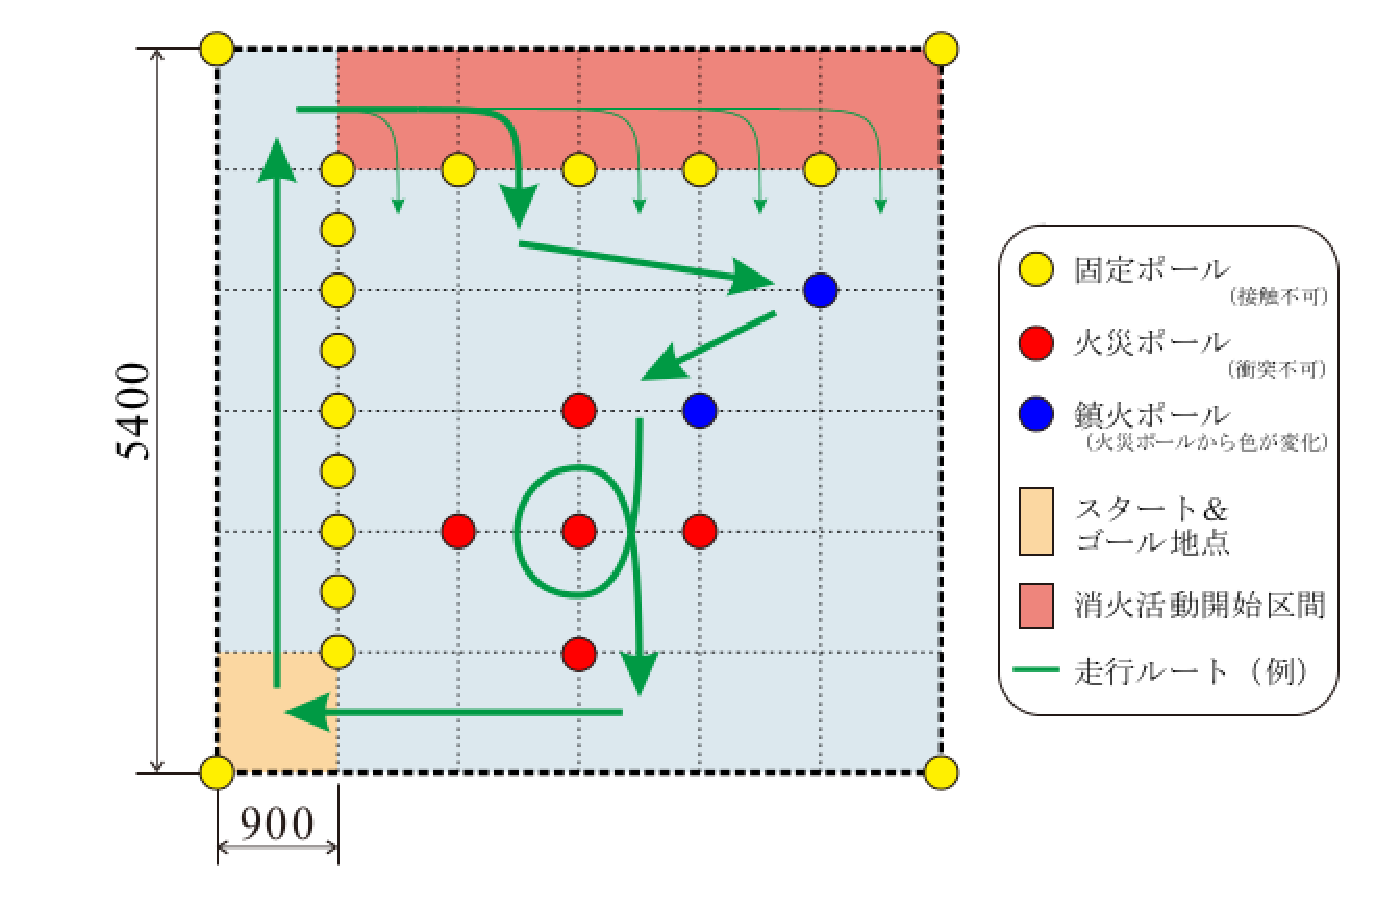
\includegraphics[width=1.0\hsize]{picture/course.eps}
    \caption{2017年度 RCR走行コース}
    \label{course}
  \end{center}
\end{figure}


\newpage
\section{ロボットカーの概要}
本年度のRCRでの我々の設計コンセプトは,
ロボットの安定した運用を可能にすることである,
そのために,ロボットカーには比較的構造が単純な独立二輪機構を採用する.
火災・鎮火ポールの判別は,ロボット前方に取り付けた単眼カメラの映像を
画像処理することで行う,また,PSD(Position Sensitive Detector)センサと
赤外線近接センサを用いてポールとロボットの距離を測定することで,
適切な軌道の走行とポールの消火を目指す.
製作にあたっては,研究室のメンバーをハードウェア,ソフトウェアの
担当に分けて進めることとする.


\section{消火について}
\subsection{消火ポール}
我々が用いる消火ポールは,以下のように製作する.\\
まず,塩化ビニル管に青い布を巻きつけて青いポールを作成する.
次に,青いポールの上から赤い布を覆うことで赤いポールとする.


\subsection{消火方法}
用いるポールの構造より,赤い布を青いポールから取り除くことで消火とする.
布を取り除く方法は,ロボットアームがポールの上から赤い布を
中に押し込んで,青いポールにするというものである.

%#MAKEINDEX makeindex interim01
\documentclass[10pt,a4j]{ujarticle}

\newcommand{\setcounters}[1] {
  \setcounter{equation}{#1}
  \setcounter{figure}{#1}
  \setcounter{table}{#1}
}

\newcommand{\unit}[1] {
  \hspace{1mm}\mathrm{[#1]}
}

\newcommand{\degc} {
  \hspace{1mm}\mathrm{[}{}^\circ\mathrm{C]}
}

\newcommand{\refig}[1]{図\ref{fig::#1}}
\newcommand{\refeq}[1]{式(\ref{eq::#1})}
\newcommand{\reftab}[1]{表\ref{tab::#1}}

\newcommand{\fig}[5] {
  \begin{figure}[#1]
    \begin{center}
      \includegraphics[width=#2\hsize]{#3}
    \end{center}
    \caption{#4}
    \label{fig::#5}
  \end{figure}
}

\makeatletter
\def\eq{\@ifstar\@eq\@@eq}
\def\@eq#1{\begin{equation*}#1\end{equation*}}
\def\@@eq#1#2{\begin{equation}#2\label{eq::#1}\end{equation}}
\makeatother

\newcommand{\diff}[2] {
  \frac{\mathrm{d}#1}{\mathrm{d}#2}
}

\newcommand{\pdiff}[2] {
  \frac{\partial #1}{\partial #2}
}


\newcommand{\ddt}[2][1] {
  \ifnum #1 < 2
    \frac{\mathrm{d}#2}{\mathrm{d}t}
  \else
    \frac{\mathrm{d}^#1#2}{\mathrm{d}t^#1}
  \fi
}

\newcommand{\e}[1] {
  \mathrm{e}^{#1}
}

\newcommand{\lparen}{(}
\catcode `( = \active
\newcommand{(}{\ifmmode\left\lparen\else\lparen\fi}

\newcommand{\rparen}{)}
\catcode `) = \active
\newcommand{)}{\ifmmode\right\rparen\else\rparen\fi}

\newcommand{\bmat}[1] {
  \begin{bmatrix} #1 \end{bmatrix}
}

% -- Package ---------------------------------------------------
\usepackage[dvipdfmx]{graphicx}
\usepackage{amsmath, amssymb}
\usepackage{bm}
\usepackage{fancyhdr}
\usepackage{here}
\usepackage{listings}
\usepackage{multirow}


% -- Margin Config ---------------------------------------------
\setlength{\textheight}{\paperheight}
\setlength{\topmargin}{4.6truemm} % 30mm(=1.0in+4.6mm)
\addtolength{\topmargin}{-\headheight}
\addtolength{\topmargin}{-\headsep}
\addtolength{\textheight}{-60truemm}

\setlength{\textwidth}{\paperwidth}
\setlength{\oddsidemargin}{-0.4truemm} % 25mm(=1.0in-0.4mm)
\setlength{\evensidemargin}{-0.4truemm}
\addtolength{\textwidth}{-50truemm}


% -- Renewcommand ----------------------------------------------
\renewcommand{\theequation}{\arabic{section}.\arabic{equation}}
\renewcommand{\thefigure}{\thesection.\arabic{figure}}
\renewcommand{\thetable}{\thesection.\arabic{table}}
\renewcommand{\lstlistingname}{ソースコード}
\renewcommand{\headrulewidth}{0mm} % fancy
\renewcommand{\labelenumi}{(\arabic{enumi})}


% -- Config for fancy package ----------------------------------
\pagestyle{fancy}
\rhead{\thepage}
\lhead{}
\cfoot{}


% -- Config for package listings -------------------------------
\lstset{
  basicstyle={\ttfamily \small},
  breaklines=true,
  frame=trBL,
  numbers=left,
  numberstyle={\ttfamily \small},
}



\begin{document}
%%%%%%%%%%%%%%%%%%%%%%%%%%%%%%%%%%%%%%%%%%%%%%%%%%%%%%%%%%%%%%%%%%%%%%
\section{消火用機構}
消火方法は前述の通りであるが,ここではそのための機構であるアーム機構について述べる.
アームは垂直方向に上下する1リンク機構を考える.これは,消火方法が布を押し込むという
単純なものであるためである.

アームの動作の概念図・並びに実際に製作したものを図\ref{arm_con},図.\ref{arm_real}に示す.
概念図のように,モータとリンクを糸状のもので接続し,モータの巻取りによって上下運動を実現する.

実際の製作では,モータを\ref{arm_real}の左のようにアームと一体化させることによって簡略化を図った.また,巻取りのリミットの判定として,アーム上部にマイクロスイッチを設置した.
\\
\\
\ \ 使用したモータは「TAMIYAミニモータ ユニバーサルギアボックス」であり,ギア比は$269:1$とした.また,回転方向の制御のためにモータドライバ「TA7291P」を使用した.

\begin{figure}[h]
 \centering
   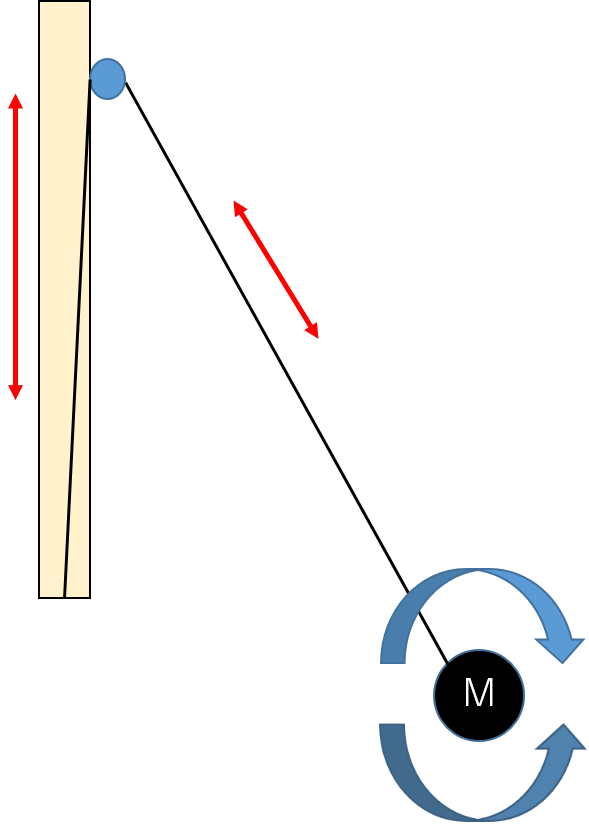
\includegraphics[clip,scale=0.4]{./picture/arm_img.png}
   \caption{消火用アーム概念図}
 \label{arm_con}
\end{figure}



\begin{figure}[h]
 \centering
 \begin{tabular}{c}

  \begin{minipage}{0.3\hsize}
   \centering
   \includegraphics[clip,scale=0.05]{./picture/side_l.png}
   \hspace{1.6cm} [1]アーム 左
  \end{minipage}
  
  \begin{minipage}{0.45\hsize}
   \centering
   \includegraphics[clip,scale=0.05]{./picture/side_r.png}
   \hspace{1.6cm} [2]アーム 右
  \end{minipage}
 \end{tabular}
 \caption{消火用アーム}
 \label{arm_real}
\end{figure}





%%%%%%%%%%%%%%%%%%%%%%%%%%%%%%%%%%%%%%%%%%%%%%%%%%%%%%%%%%%%%%%%%%%%%%%%%%%%
\end{document}

\section{PSDセンサの同定実験}
\label{psdex}

前年度までに研究室で購入していた2種類のPSDセンサについて,
そのPSDセンサの精度を確かめるために同定実験を行った.

\subsection{センサの仕様}
前年度までに購入していた2種類のPSDセンサの仕様を以下に示す.
また,下記2つのセンサを便宜上,順に近距離センサ,遠距離センサと
呼ぶこととする.\\

 \begin{description}
  \item[【シャープ測距モジュール GP2Y0A21YK】] \mbox{} \\
	     測距範囲:$10〜80\unit{cm}$ \\
	     出力:アナログ電圧出力 \\
	     寸法:$29.5×13×13.5\unit{mm}$ \\
	     電源:$4.5〜5.5\unit{V}$
  \item[【シャープ測距モジュール GP2Y0A02YK】] \mbox{} \\
	     測距範囲:$20〜150\unit{cm}$ \\
	     出力:アナログ電圧出力 \\
	     寸法:$29.5×13×21.6\unit{mm}$ \\
	     電源:$4.5〜5.5\unit{V}$
 \end{description}


\subsection{実験装置}
PSDセンサの実験を行うため,図\ref{psded}のような実験装置を製作した.
PSDセンサは高さ$20\unit{mm}$の位置にセンサの発光部が左,
受光部が右になるように箱に水平に装着した.
PSDセンサを動作せるのにはArduino Unoを用い,
Arduino IDEのシリアルモニタを用いて出力電圧を測定した.
実験時のセンサとArduinoの配線を図\ref{psdwd}に,
Arduinoのプログラムを付録1に示す.
配線にはブレッドボードを用いた.また,ポールの代わりに,
ポールと同じ形状のスプレー缶を用いた.

\begin{figure}[t]
  \begin{center}
   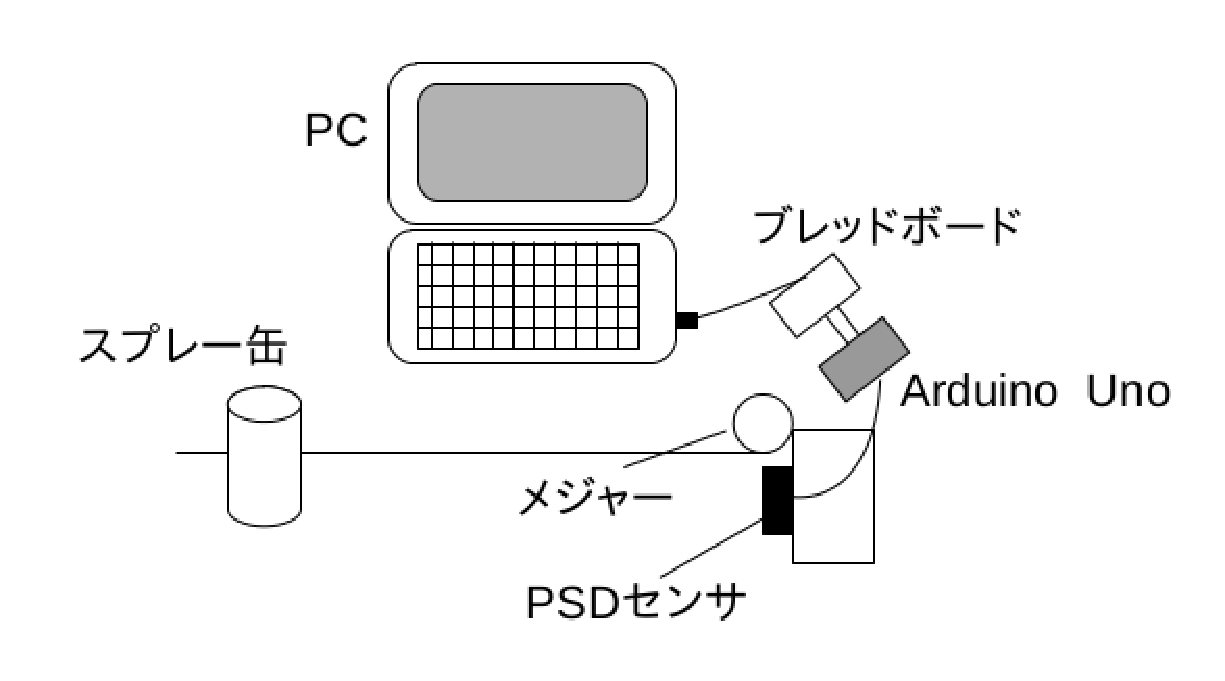
\includegraphics[scale = 0.8]{picture/psded.eps}
   \caption{PSD実験装置}
   \label{psded}
  \end{center}
\end{figure}

\begin{figure}
 \begin{center}   
  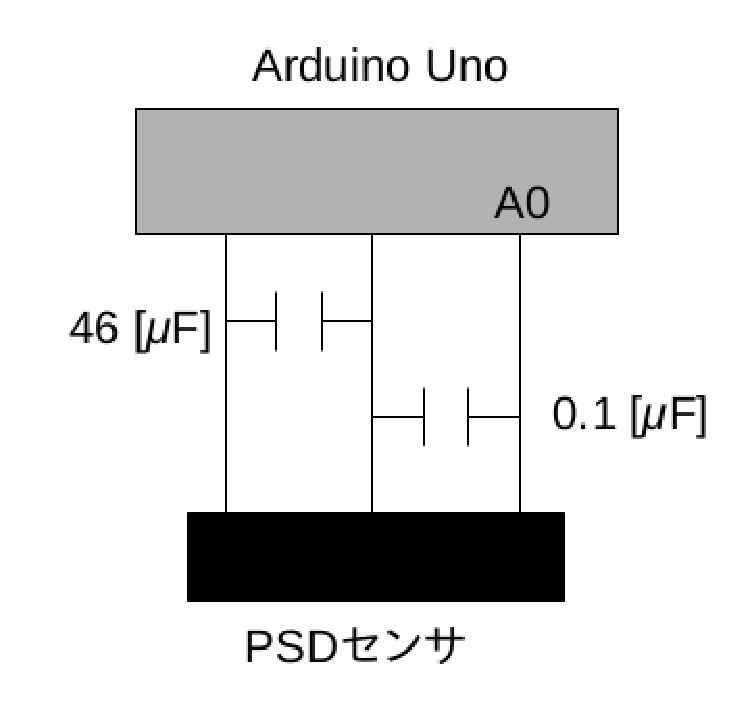
\includegraphics[scale = 0.8]{picture/psdwd.eps}
  \caption{PSDセンサの配線図}
  \label{psdwd}
 \end{center}
\end{figure}


\newpage
\subsection{実験方法}
PSDセンサの距離-出力電圧特性を測定するため以下の手順に従い実験を行った.
\begin{enumerate}
 \item PSDセンサの発光部・受光部の先端を距離$0\unit{cm}$とし,
       近距離センサは$5\unit{cm}$から$100\unit{cm}$まで,
       $5\unit{cm}$ずつスプレー缶を移動させ出力電圧を記録する.
       このとき,スプレー缶の中心はPSDセンサの中心の正面にくるように
       置き測定する.
 \item 先程と同様に,遠距離センサは$5\unit{cm}$から$170\unit{cm}$まで,
       $5\unit{cm}$ずつスプレー缶を移動させ出力電圧を記録する.
\end{enumerate} 

\subsection{実験結果}
縦軸を出力電圧,横軸をPSDセンサ-スプレー缶間の距離とし,
近距離センサの測定結果のグラフを図\ref{psdn}に,
遠距離センサの測定結果のグラフを図\ref{psdf}に示す.
図\ref{psdn}より,近距離センサは出力電圧が$40\unit{cm}$までは
滑らかに減少しており,$40\unit{cm}$からは大きな変化は見られない.
それに対して図\ref{psdf}より,遠距離センサは測距可能範囲内において
出力電圧が$80\unit{cm}$までは滑らかに減少しており,
$80\unit{cm}$からは変化に乏しいことがわかる.
よって,近距離センサでは$40\unit{cm}$以降,遠距離センサでは$80\unit{cm}$以降の距離を算出することが難しくなると考えられる.
ここで,今回のロボットは$40\unit{cm}$以降も距離を計測する必要がある.
従って適当なセンサは,遠距離センサであると考えられる.


\newpage
\begin{figure}[htb]
  \begin{center}
    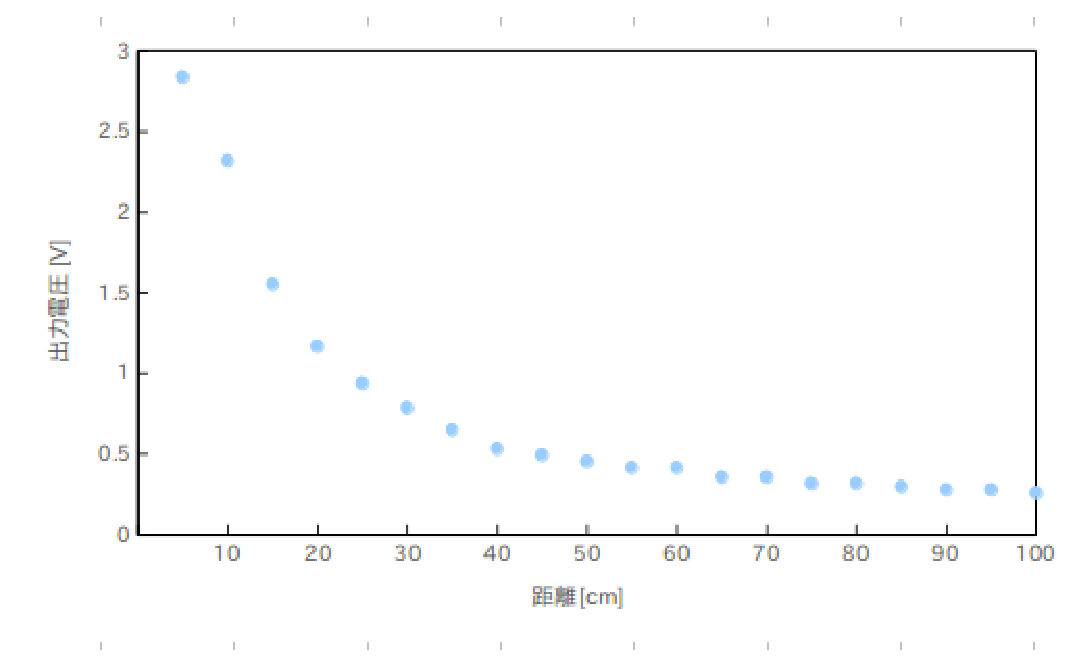
\includegraphics[width=1.0\hsize]{picture/psdn.eps}
    \caption{近距離センサ}
    \label{psdn}
  \end{center}
\end{figure}

\begin{figure}[H]
  \begin{center}
    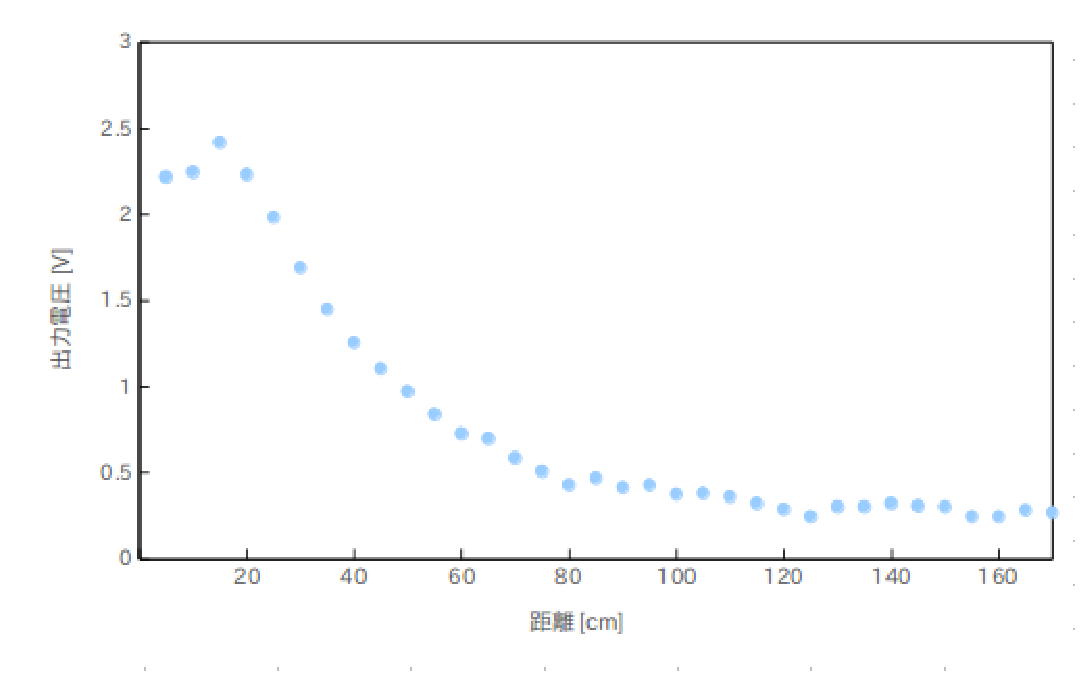
\includegraphics[width=1.0\hsize]{picture/psdf.eps}
    \caption{遠距離センサ}
    \label{psdf}
  \end{center}
\end{figure}


\newpage

\section{機体の再設計}
\subsection{前回の反省}
第1回のレポートで紹介した機体を図\ref{kuwano1}に示す.これを一号機とし,
一号機での反省点を元に再設計した機体を二号機とした.
二号機の概要を図\ref{kuwano2}に示す.一号機での反省点を以下に述べる.

\begin{itemize}
 \item 車体に無駄なスペースが多い.
 \item 車体の幅が大きい.
 \item 回路のガードがされていない.
\end{itemize}

西田研究室では,これらの反省点を改善するために,機体の大幅な見直しを行った.
改善した点について以下に述べていく.

\subsection{モータとエンコーダの配置}
一号機の駆動系を図\ref{kuwano3}に示す.一号機では,
モータとエンコーダの配置を線対称としていたため,
機体の幅が大きくしなければならなかった.そこで,
二号機ではこのモータとエンコーダの配置を点対象とすることにした.
これにより,タイヤのトレッド幅を限りなく小さくでき,
機体の幅を小さくすることができた.
また,一号機ではモータとエンコーダをアルミ板で下から支えるようになっていた.
そのため,モータとエンコーダを支える以外のスペースは無駄なスペースとなっていた.
二号機ではこの無駄なスペースを省くために,
モータとエンコーダを上から支えることにした.上から支えるにしたがって,
モータとエンコーダの重量と機体の荷重が図\ref{kuwano4}に示した部分に集中する恐れがあるため
,機体中心部分にモータおよびエンコーダを支えるパーツを3Dプリンタで作成し,
設置した.以上より,下から支えていたアルミ板を廃止することができ,
一号機での無駄なスペースを削減することができた.

\subsection{回路のガードについて}
機体の大部分はアルミでできているため,回路をそのままにしておくと,
ショートする可能性がある.したがって,回路をホットボンドで覆うことで
ショートすることを防ぐようにした.Arduinoに関しては専用のケースが存在しないため,
3Dプリンタでケースを作成した.

\subsection{タイヤについて}
一号機では図\ref{kuwano5}のようなタイヤを使用していたが,
このタイヤは中身がスポンジになっており,機体の重量でタイヤの接地面積が増えやすく,
また機体の荷重移動によって機体がロールする可能性があると考えた.
二号機ではそういった問題を解消するべく,ナロータイヤを使用することにした.
使用するナロータイヤを図\ref{kuwano6}に示す.使用するナロータイヤは非常に細いため,
地面との接地面積を少なくすることができる.また,ゴムのみでできているので,
一号機で使用する予定であったタイヤに比べて沈む量が少なく,
機体の荷重移動によるロールも低減できると考えられる.
しかし,接地面が小さくなったことでスリップする可能性があると考えられるので,
キャンバー角をつけるなどして対策を考えていく.

\begin{figure}[H]
  \begin{center}
    \includegraphics[width=1.0\hsize]{../../report_2/kuwano/picture/kuwano1.eps}
    \caption{一号機}
    \label{kuwano1}
  \end{center}
\end{figure}

\begin{figure}[H]
  \begin{center}
    \includegraphics[width=1.0\hsize]{../../report_2/kuwano/picture/kuwano2.eps}
    \caption{二号機}
    \label{kuwano2}
  \end{center}
\end{figure}

\begin{figure}[H]
  \begin{center}
    \includegraphics[width=1.0\hsize]{../../report_2/kuwano/picture/kuwano3.eps}
    \caption{一号機の駆動系}
    \label{kuwano3}
  \end{center}
\end{figure}

\begin{figure}[H]
  \begin{center}
    \includegraphics[width=1.0\hsize]{../../report_2/kuwano/picture/kuwano4.eps}
    \caption{最も荷重がかかる位置}
    \label{kuwano4}
  \end{center}
\end{figure}

\begin{figure}[H]
  \begin{center}
    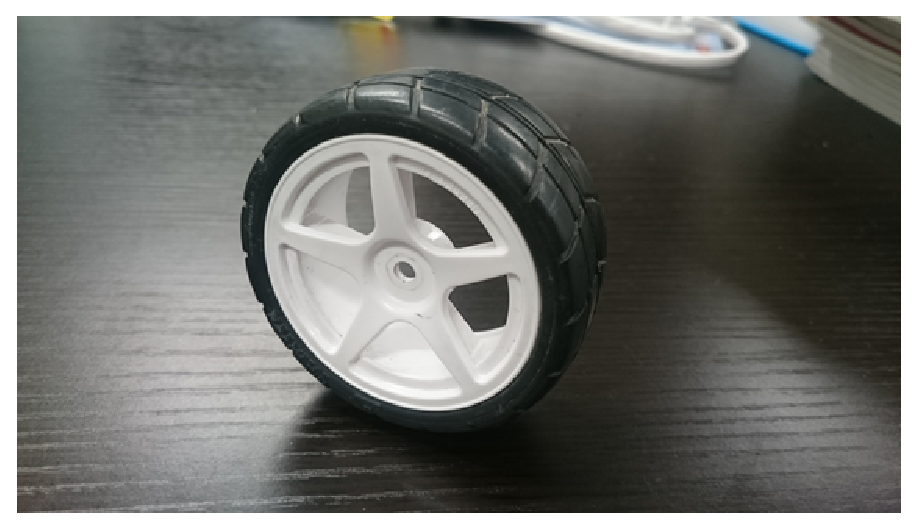
\includegraphics[width=1.0\hsize]{../../report_2/kuwano/picture/kuwano5.eps}
    \caption{一号機のタイヤ}
    \label{kuwano5}
  \end{center}
\end{figure}

\begin{figure}[H]
  \begin{center}
    \includegraphics[width=1.0\hsize]{../../report_2/kuwano/picture/kuwano6.eps}
    \caption{二号機のナロータイヤ}
    \label{kuwano6}
  \end{center}
\end{figure}

\subsection{第二回中間発表のデモ走行について}
第二回中間発表でデモ走行を行ったが,途中で停止してしまった.本機体は四点で支えられており,
路面の凹凸によって三点しか接地できなかった場合に機体が「やじろべえ」と同じような状態になってしまい,
駆動力が路面に十分に伝わらず停止したと考えた.

\subsubsection{実地調査}
この問題を解決する前に,我々はRCRの会場(記念講堂)においても今回と同じような問題が生じるのかを
確かめることにした.実地調査をするためには機体を自由に動かせる必要があるため,
機体をワイヤレスコントローラ (DUALSHOCK3)を用いて動かせるようにした.記念講堂で動かしてみた結果,
途中で機体が停止することはなかったため,機体に修正を加える必要はないと考えた.

\section{回路設計}
設計した回路について選定の理由や仕様について以下に示す.
また使用する部品の一覧を表\ref{tab:c_parts}に示す.

\subsection{マイコンの選定}
設計した回路を図\ref{c_raspberry},図\ref{c_arduino}に示す.
マイコンとして「Raspberry Pi3 Model B(以下 RPi)」と「Arduino uno R3(以下 Arduino)」を使用する.それぞれが,統合・画像処理・モータ制御,
センサ処理,を行う.RPiでは複雑な処理を行う上で,LinuxOSの支援を受けることができ有利である.さらに,処理速度がCPU 1.2[GHz],
メモリ1[GB]とArduinoの16[MHz]・32[KB]と比べても大きく優れている.これは,並列処理や高速な画像処理に適している.このような理由からRPi
を採用した.

また ,RPiはアナログI/Oポートを持っておらず,アナログ電圧出力を行うセンサ類の処理が困難である.そこで,アナログ・ディジタルI/Oポートを
持つArduinoにセンサ類の処理を担わせることとした.ただし,要求されるアナログI/Oポート数が後述の$I^2 C$通信を使用しても足りない.そこで
Arduino用16チャンネル・アナログ・マルチプレクサを使用することで増設を行った.
\begin{table}[H]
  \centering
  \caption{回路用部品表}
  \begin{tabular}{|l|l|r||l|} \hline
    タイプ & 部品名 & 数 & 用途 \\ \hline \hline
     マイコン & Raspberry Pi3 & 1& 統括・画像処理・モータ制御 \\ \cline{2-4}
     & Arduino uno R3& 1 & センサ類の処理 \\ \hline
     DCモータ & AO-8014 & 2 & 駆動用 \\ \cline{2-4}
      & TAMIYA ミニモータ & 1&アーム用  \\ \hline
    モータドライバ& MD10C-R3 & 2& タイヤ用 \\ \cline{2-4}
      &  TA7291P&1 &アーム用 \\ \hline
   アナログマルチプレクサ & CD74HC4067 & 1 & ArduinoアナログI/Oピン増設 \\ \hline
    $I^2 C$通信用変換モジュール&PCA9306&1&$I^2 C$通信\\ \hline
     赤外線測距センサ& GP2Y0A02YK &6&中距離センサ\\ \hline
      ToF近距離センサ& VL6180x&3&近接センサ \\ \hline
     カメラモジュール&P5V04A&1&画像処理\\ \hline
     3軸加速度センサ&KXR94-2050&1&自己位置推定\\ \hline
     3軸ジャイロセンサ&BGD20&1&自己位置推定\\ \hline
    DCDCコンバータ&LT8697&1& 7.2[V]→5.0[V]2500[mA]降圧レギュレータ\\ \cline{2-4}
       &BTD05-05S200D&1&7.2[V]→5.0[V]2000[mA]降圧レギュレータ\\ \hline
    コンデンサ&電解コンデンサ 47[$\mu$F]&2&電源安定化\\ \cline{2-4}
            &セラミックコンデンサ 0.1 $\mu$ ]&9&センサ信号安定化\\ \hline
   バッテリー&POWER MAX 4000 Ni-MH&1&電源バッテリー 7.2[V]4200[mAh]\\ \hline
                 
  \end{tabular}
  \label{tab:c_parts}
\end{table}
\newpage
\begin{figure}[H]
 \centering
 \includegraphics[clip,scale=0.35]{../../report_2/kakeru/picture/raspberryPi3.eps}
 \caption{Raspberry Pi3 接続回路図}
 \label{c_raspberry}
\end{figure}

\begin{figure}[H]
 \centering
 \includegraphics[clip,scale=0.35]{../../report_2/kakeru/picture/arduino_02.eps}
 \caption{Arduino unoR3 接続回路図}
 \label{c_arduino}
\end{figure}
\newpage

%%%%%%%%%%%%%%%%%%%%%%%%%%%%%%%%%%%%%%%%%%%%%%%%%%%%%%%%%%%%%%%%%%%%%%%%%%%%%%%%%%%%%%%%%%%
\subsection{モータドライバ}
モータドライバは「MD10C R3」(図\ref{MD10C})を両輪駆動用として2つ使用し,
「TA7291P」(図\ref{TA7291P})をアーム用として使用する.
各仕様を下に示す.

[MD10C R3](駆動用)
\begin{itemize}
 \item モータ電源電圧 : DC 5[V]$〜$25[V]
 \item モータ最大電流 : 13[A]
 \item ロジック用電源 : モータ用より供給
 \item ロジック電圧   : DC 5[V] or 3.3[V]
\end{itemize}

[TA7291P](アーム用)
\begin{itemize}
 \item モータ電源電圧 : DC 0[V]$〜$20[V]
 \item モータ最大電流 : 1.0[A]
 \item ロジック電圧 : DC 4.5[V]$〜$20[V]
\end{itemize}
\begin{figure}[H]
 \centering
 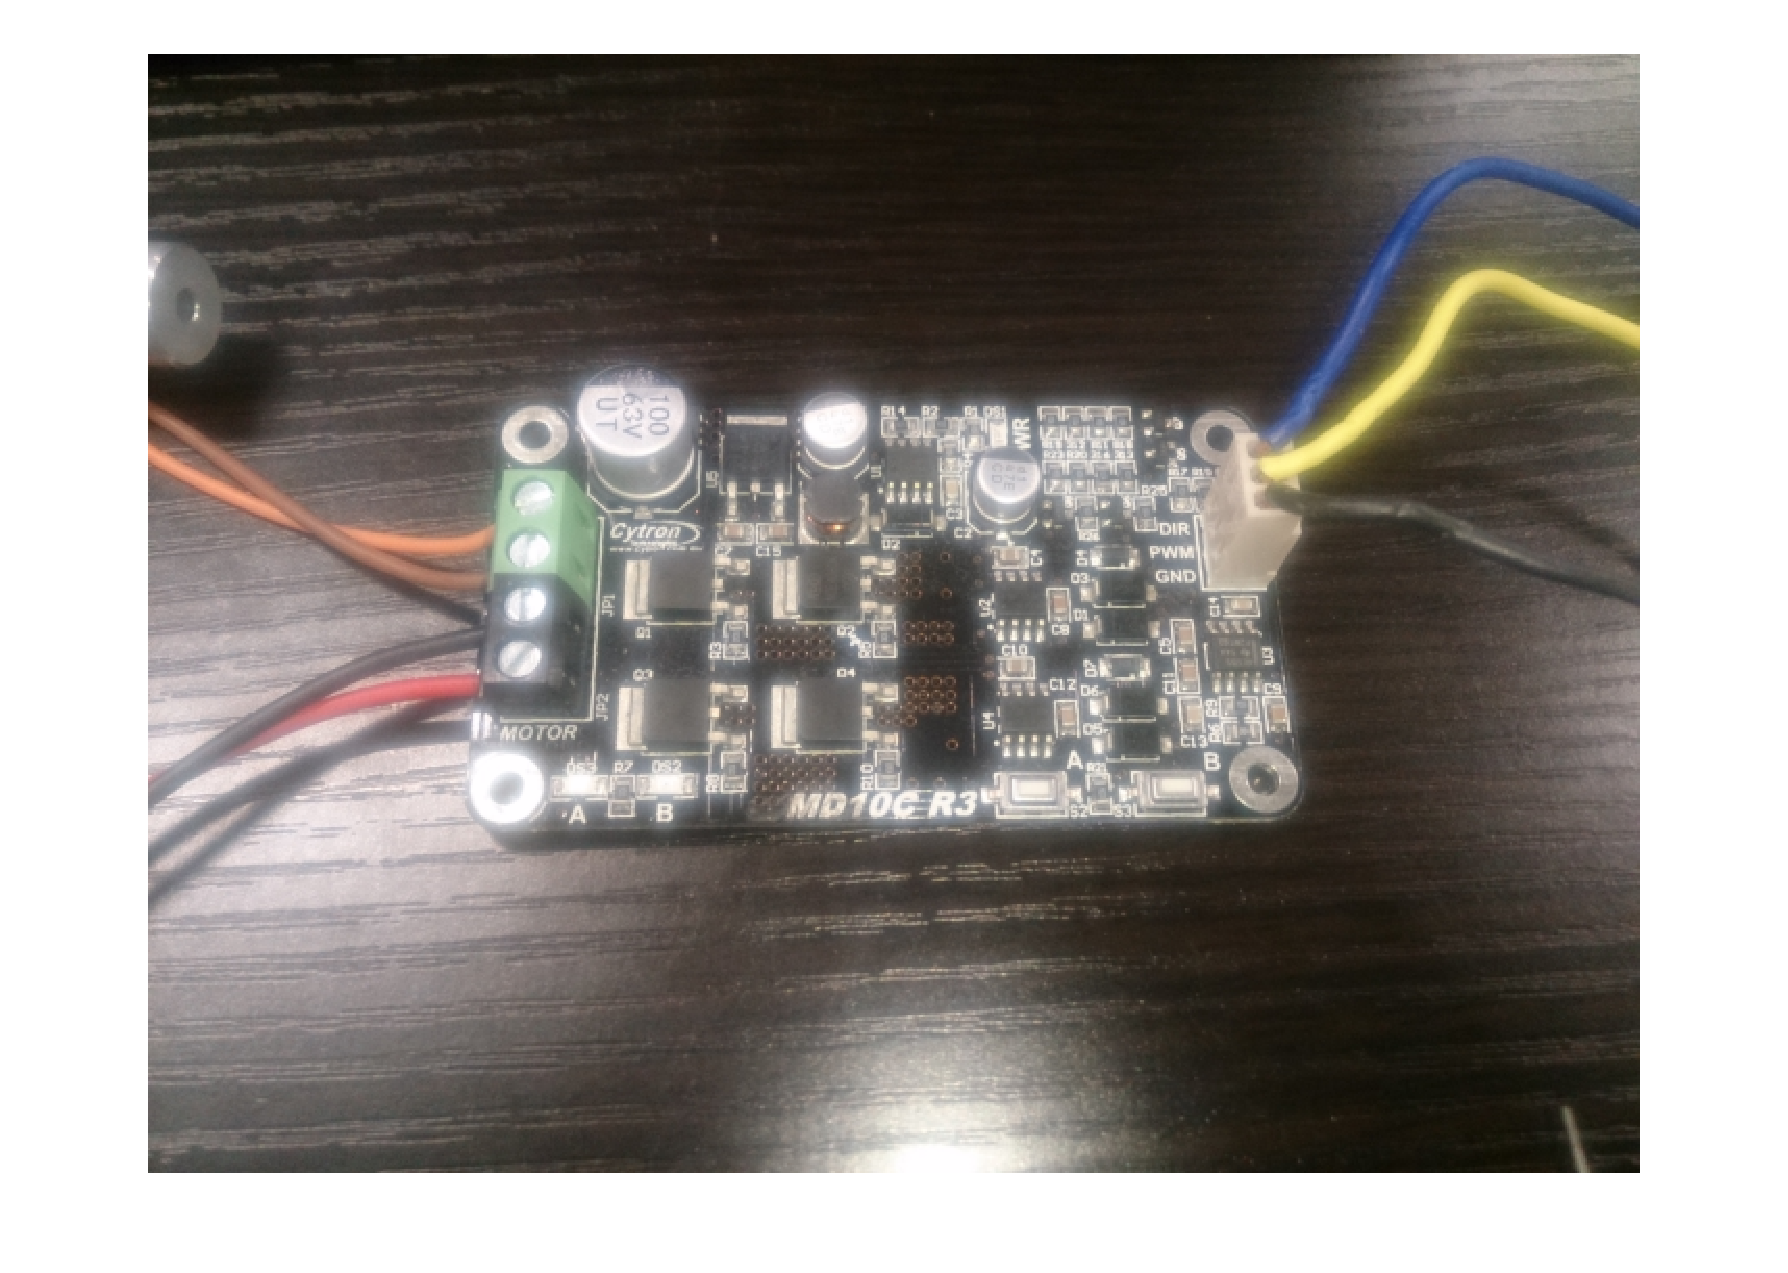
\includegraphics[width=0.5\hsize]{../../report_2/kakeru/picture/MD10C.eps}
    \caption{MD10C R3}
    \label{MD10C}
\end{figure}
\begin{figure}[H]
 \centering
 \includegraphics[width=0.5\hsize]{../../report_2/kakeru/picture/TO.eps}
    \caption{TA7291P}
    \label{TA7291P}
\end{figure}

%%%%%%%%%%%%%%%%%%%%%%%%%%%%%%%%%%%%%%%%%%%%%%%%%%%%%%%%%%%%%%%%%%%%%%%%%%%%%%%%%%%%%%%%%%%%%%

\subsection{センサ仕様}
ロボットに搭載されているセンサは以下である.
\begin{itemize}
 \item 赤外線測距センサ : GP2Y0A025YK : 有効距離$20 〜 150$[cm]
 \item ToF近距離センサ : VL6180x    : 有効距離$5 〜 20$[cm]
 \item 3軸加速度センサ : KXR94-2050 : [ x, y, z ]軸 加速度出力
 \item ジャイロセンサ : L3GD20 : [ x, y, z ]軸 角加速度出力
 \item カメラモジュール : P5V04A : RPi用カメラ
\end{itemize}
%%%%%%%%%%%%%%%%%%%%%%%%%%%%%%%%%%%%%%%%%%%%%%%%%%%%%%%%%%%%%%%%%%%%%%%%%%%%%%%%%%%%%%%%
\subsubsection{測距センサ}  
測距センサは本体周囲にPSDセンサを7つ,前方にToF近接センサを3つ搭載する.(図\ref{Distance})これは自律行動の際に,
周辺環境,特に各種ポールを把握するために用いる.このとき,近接センサは$I^2 C$通信によって使用する.
センサの仕様については実験を行ったので\ref{psdex}に示す.

また,各測距センサには信号のノイズを吸収し安定化させるために$0.1[\mu $F]のセラミックコンデンサを接続する.
これは,コンデンサの持つ交流成分のみを吸収し,直流成分を通すというローパスフィルタ的特徴を利用したものである.

\begin{figure}[b]
 \centering
 \includegraphics[width=0.5\hsize]{../../report_2/kakeru/picture/Distance.eps}
    \caption{上:PSDセンサ 下:ToFセンサ}
    \label{Distance}
\end{figure}
%%%%%%%%%%%%%%%%%%%%%%%%%%%%%%%%%%%%%%%%%%%%%%%%%%%%%%%%%%%%%%%%%%%%%%%%%%%%%%%%%%%%%%%%%%%%
\subsubsection{3軸加速度・ジャイロセンサモジュール}
加速度センサは[ x, y, z ]軸におけるロボットの加速度を測定するものである.

ジャイロセンサは[ x, y, z ]軸まわりの角加速度を測定するものである.(図\ref{jairo})

我々はこれらをロボットの自己位置推定に用いる.特にジャイロセンサについては,
ロボット本体の直進走行制御に使用する.詳細は\ref{algo}において説明する.
\begin{figure}[t]
 \centering
 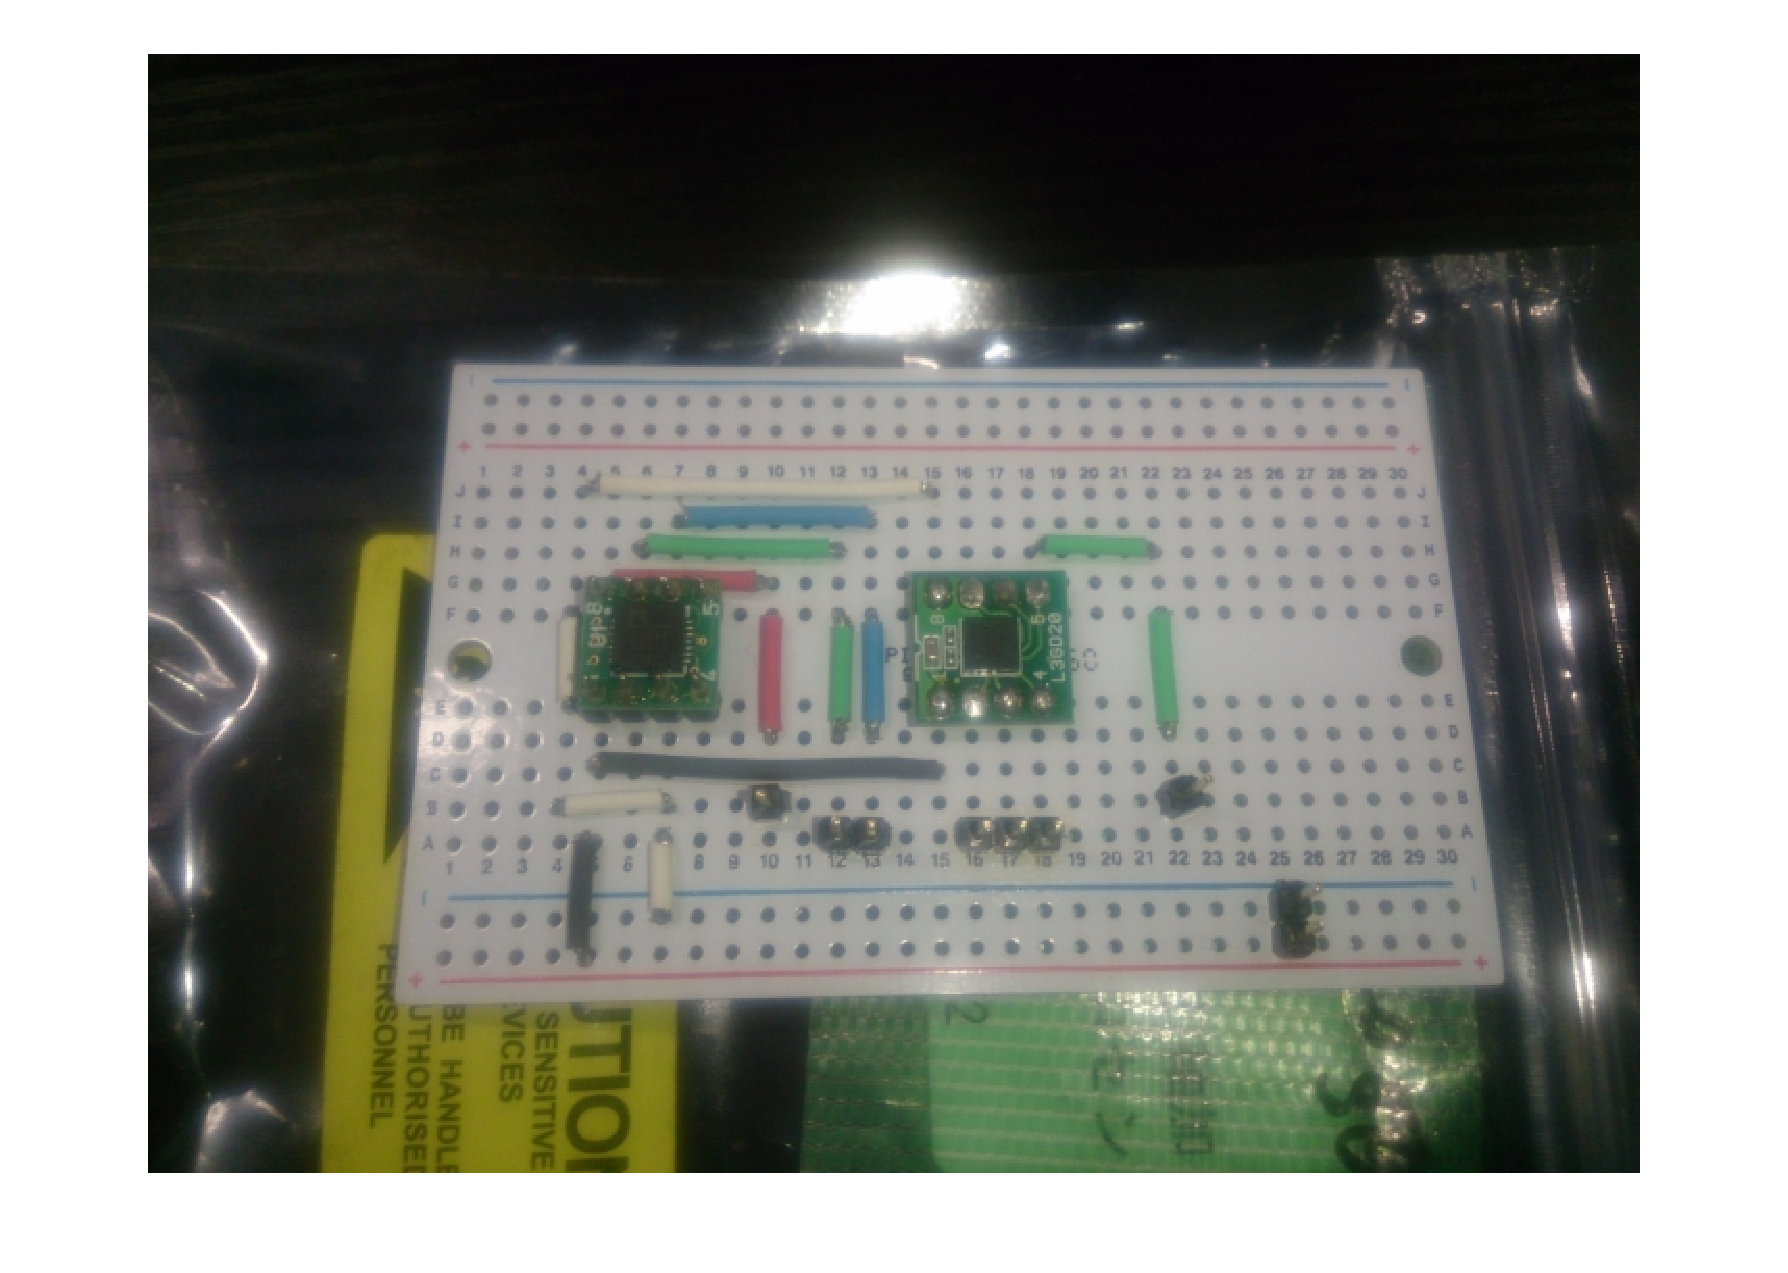
\includegraphics[width=0.4\hsize]{../../report_2/kakeru/picture/jairo.eps}
    \caption{3軸加速度・ジャイロセンサモジュール}
    \label{jairo}
\end{figure}

\subsection{電源回路}
電源回路は各回路図の左上に示している.\\
バッテリーはひとつしか搭載しないが,RPiとArduinoでは定格電流値が異なるために同一の電源は使用できない.
そこで,それぞれに降圧レギュレータとしてDCDCコンバータを用いてバッテリーからの供給電源を
分電することとした.各仕様を下に示す.
また,実際に作成した電源回路を図\ref{dengen}に示す.

[LR8697](RPi・モータ用)
\begin{itemize}
 \item 電源電圧 : DC 6.0[V]$〜$42.0[V]]
 \item 出力電圧 : DC 5.0[V]]
 \item 出力電流 : 2.5[A]
\end{itemize}

[BTD05-05S200D](Arduino・センサ用)
\begin{itemize}
 \item 電源電圧 : 4.5-9.0[V]
 \item 出力電圧 : 5.0[V]
 \item 出力電流 : 2000[mA]
\end{itemize}
\begin{figure}[t]
 \centering
 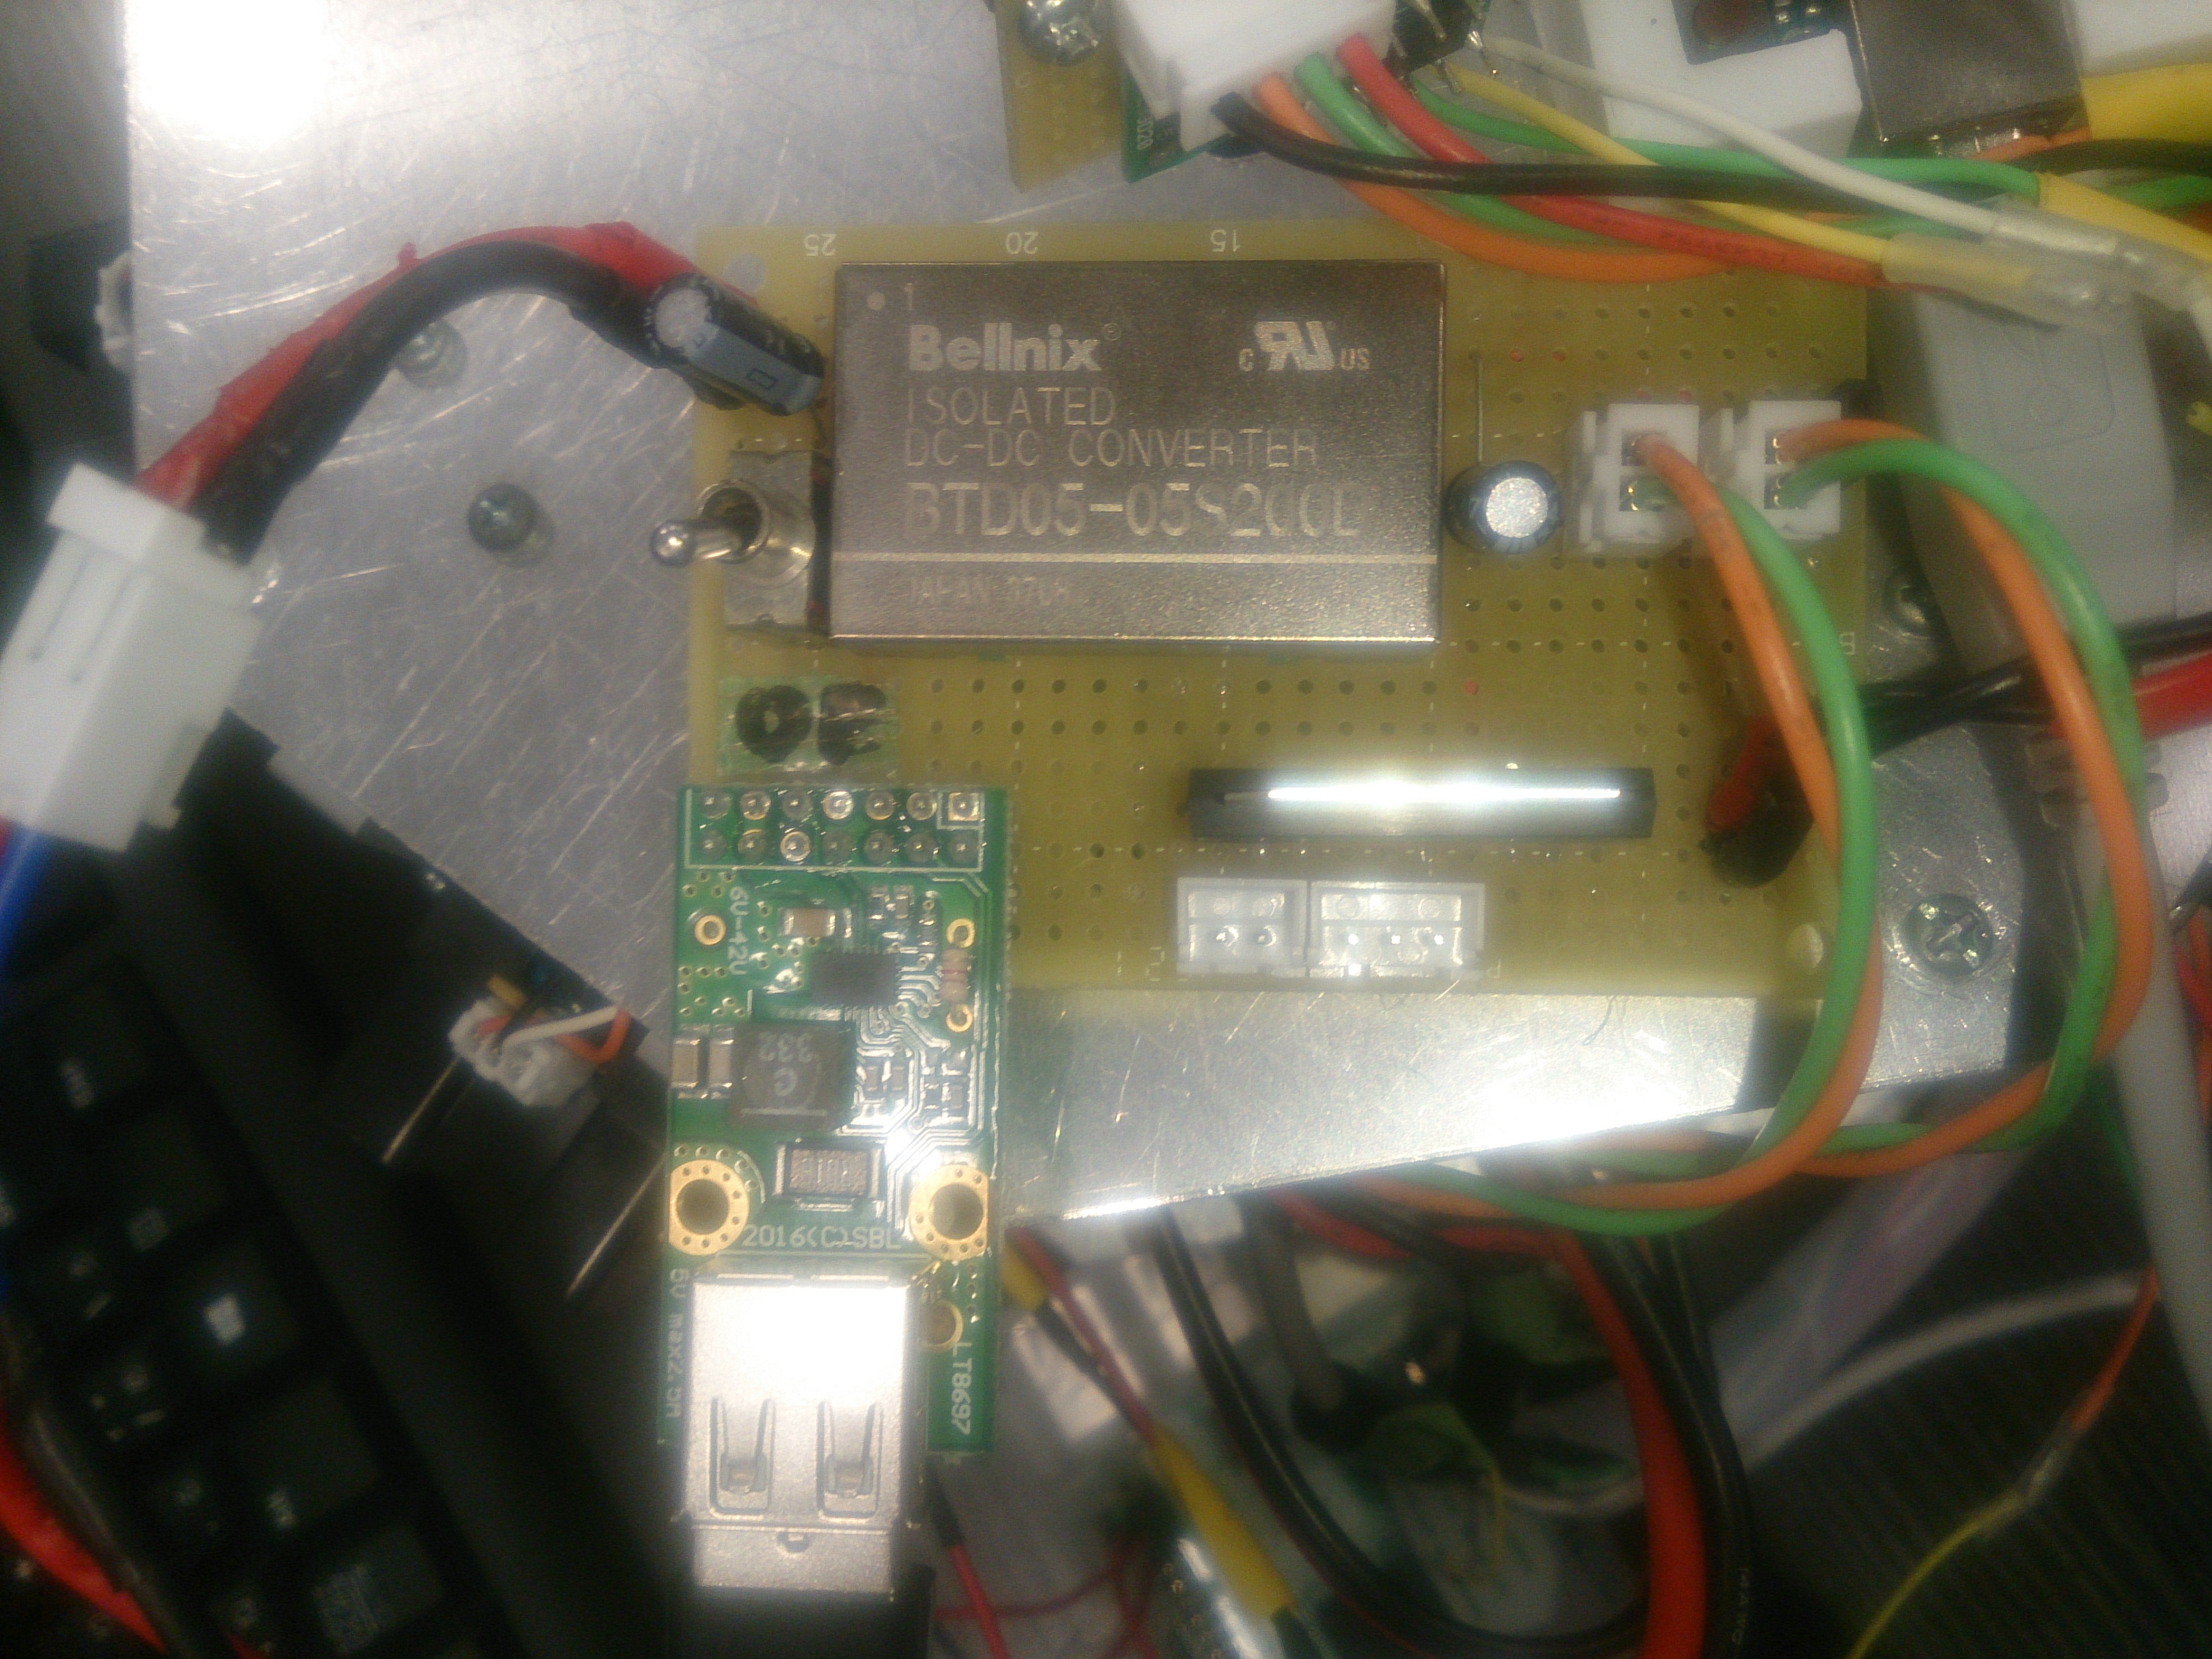
\includegraphics[width=0.4\hsize]{../../report_2/kakeru/picture/dengen.eps}
    \caption{電源回路モジュール}
    \label{dengen}
\end{figure}
%%%%%%%%%%%%%%%%%%%%%%%%%%%%%%%%%%%%%%%%%%%%%%%%%%%%%%%%%%%%%%%%%%%%%%%%%%%%%%%%%%%%%%%%%%%
\newpage
\subsection{$I^2 C$通信}
今回,我々のロボットには測距センサを始めとする複数のセンサが搭載されている.これらの殆どがアナログ出力
であるが,ArduinoのアナログI/Oポートは6つしかなく,要求を満たしていない.

そこで,$I^2 C$通信を用いることとする.これは,$I^2 C$通信がパーティライン構成が可能となっており
,1つのマスタで複数のスレーブデバイスと通信することが可能であるからである.概要を以下に示す.
\begin{enumerate}
 \item マスタ側(Arduino)とスレーブ側(n個のセンサ等)を明確に分け,各スレーブに異なるアドレスを割り振る.
 \item マスタ側が、Start Conditionを出力し続いてアドレスとRead/Write要求を出力する.
 \item 全スレーブがこの時のSCLのクロックを元にSDAのデータを受信し、SSPADDレジスタにセットされたアドレスと一致したデバイスだけが、その後の送受信を継続する.
 \item 受信した側がデータを受信完了すると自動的にACKビットを返送し、同時にSSP割込みを発生する.
 \item これをマスタがStop Conditionを出力するまで続ける.
\end{enumerate}

本ロボットでは,近接センサ・ジャイロセンサについて$I^2 C$通信を行うこととする.また,Arduinoと各デバイスは
ArduinoのSDA・SCLポートを使用することで通信が可能となる.これを実現するためにArduino用$I^2 C$バス用双方向電圧レベル変換モジュール
(図\ref{level})を使用して接続した.接続の方法は回路図に示している.

\begin{figure}[b]
 \centering
 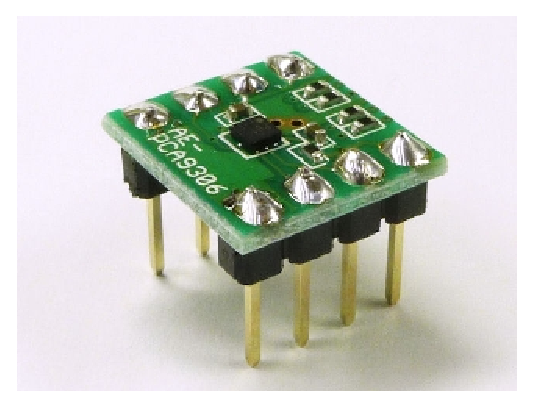
\includegraphics[width=0.4\hsize]{../../report_2/kakeru/picture/level.eps}
    \caption{レベル変換モジュール}
    \label{level}
\end{figure}


\newpage

\section{ソフトウェア}
\subsection{モデル化}
プログラム上でセンサから読み取った値を扱えるようにするため,モデル化を行った.
ここでの距離,加速度,電圧の単位はそれぞれcm,$\mathrm{m}/\mathrm{s}^{2}$,Vである.

\subsubsection{PSDセンサ GP2Y0A21}
前回求めたPSDセンサの性能から距離-電圧特性は以下のようになる.
\begin{equation}
 (距離)=45.514×(電圧)^{-0.822}
\end{equation}

\subsubsection{近接センサ VL6180X}
前回のPSDセンサと同様な実験で,近接センサの距離と出力値の関係を求めた.
そのときの関係を表した式を以下に示す.
また,出力値とはarduinoで0〜255までの値で出力された値であり,
対象物との距離が近いほど,値が小さくなるようにプログラムで処理している.
\begin{equation}
 (距離)=0.09999×(出力値)+0.4477
\end{equation}

\subsubsection{加速度センサ KXR-94 }
この加速度センサのモデル化するために必要な仕様を以下に示す.
\begin{itemize}
 \item 感度:1 [V/g]
 \item オフセット:2.5 [V]
\end{itemize}

これらより,加速度と電圧の関係を以下に示す.
\begin{equation}
 (加速度)=9.8×[(電圧)-2.5]
\end{equation}


\subsection{フィルタ処理}
   \subsubsection{ローパスフィルタ}
 加速度センサやジャイロセンサで読み取った値は,ノイズが入り大きく上下していた.
そこでセンサ値の平滑化を行うため,ローパスフィルタを用いた.ローパスフィルタの式は以下に示す.

\begin{equation}
 y[i]=py[i-1]+(1-p)x[i]
 \label{low_pass}
\end{equation}
ここで,$y[i]$は出力値,$y[i-1]$は前回の出力値,$x[i]$は現在のセンサ値であり,
$p(0<p<1)$はパラメータである.この式の特徴として,パラメータ$p$を大きくすれば滑らかになるが,
位相が遅れることがわかっている.

   \subsubsection{ハイパスフィルタ}
センサ値をローパスフィルタで平滑化を行い,移動距離や回転角度を求めるためにその値の積分を行った.
ここでの積分は数値積分であったため,積分誤差が生じ,時間とともに値がずれていた.
これを解決するためにハイパスフィルタを用いた.ハイパスフィルタの式は以下に示す.

\begin{equation}
 \acute{y}[i]=x[i]-y[i]
 \label{high_pass}
\end{equation}
ここで,$\acute{y}[i]$は出力値,$x[i]$は現在の積分したセンサ値,
$y[i]$は積分したセンサ値をローパスフィルタに通した出力値である.

\subsection{自己位置推定}
   \subsubsection{アフィン変換}
   加速度センサで得られる加速度はロボットのローカル座標系における加速度である.そこで,ジャイロセンサから得られた角度を用いて三次元アフィン変換を適用しグローバル座標系における加速度を求める.\\
   アフィン変換において,回転移動は次の行列で表される.$x$軸,$y$軸,$z$軸まわりの回転行列をそれぞれ$R_x, R_y, R_z$とおくと,
   \begin{eqnarray}
    R_x = \left[
	   \begin{array}{cccc}
	    1 &        0      &       0       & 0 \\
	    0 & \cos \theta_x & \sin \theta_x & 0 \\
	    0 & -\sin \theta_x& \cos \theta_x & 0 \\ 
	    0 &        0      &       0       & 1 
	   \end{array}
	  \right] \\
    R_y = \left[
	   \begin{array}{cccc}
	    \cos \theta_y & 0 & -\sin \theta_y & 0 \\
	          0       & 1 &       0        & 0 \\
	    \sin \theta_y & 0 &  \cos \theta_y & 0 \\ 	
	          0       & 0 &       0        & 1 
	   \end{array}
	  \right] \\
    R_z = \left[
	    \begin{array}{cccc}
	     \cos \theta_z & \sin \theta_z & 0 & 0 \\
	    -\sin \theta_z & \cos \theta_z & 0 & 0 \\
		   0	   &	   0	   & 1 & 0 \\ 	
	           0       &       0       & 0 & 1 \\
	    \end{array}
	   \right] 
   \end{eqnarray}
   また,ローカル座標系の原点のグローバル座標系での座標を$(T_x,T_y,T_z)$とすると,アフィン変換における平行移動は次の行列で表される.
   \begin{equation}
    T = \left[
	    \begin{array}{cccc}
	      1  &  0  &  0  & 0 \\
	      0  &  1  &  0  & 0 \\
	      0  &  0  &  1  & 0 \\ 	
             T_x & T_y & T_z & 1 \\
	    \end{array}
	   \right]     
   \end{equation}
   ここで,ローカル座標系を$(x,y,z,1)$,グローバル座標系を$(x_g,y_g,z_g,1)$とすると
   \begin{equation}
    (x_g \  y_g \ z_g \ 1) = (x \ y \ z \ 1) R_z  R_x  R_y T
   \end{equation}
   となる.これによってローカル座標系の加速度センサで得られた加速度をグローバル座標系に変換することができた.
   
   \subsubsection{ジャイロセンサ}
   ジャイロセンサ(角速度センサ)を用いて,車体の角度を求める.
角速度センサと同様に考える.
角度を$\theta(t)$[deg],角速度を$\omega(t)$[deg/s]とすると

\begin{equation}
 \theta(t)=\frac{t_2-t_0}{6}(\omega(t_0)+4\omega(t_1)+\omega(t_2) )
\end{equation}
となる.

\subsubsection{加速度センサ}
加速度センサを用いて,移動距離を求める.
そのために加速度センサから,加速度とそのときの時間を得る.
今回は加速度を積分するのに,数値積分のシンプソン公式を用いた.
シンプソン公式による区間$(a,b)$の$f(t)$の積分値は以下のようになる.


\begin{equation}
 \int_a^b f(t) dt = \frac{b-a}{6} ( f(a)+4f ( \frac{a+b}{2}) +f(b))
\end{equation}

これを用いて,$(t_0,t_2)$の区間で積分する(ただし$t_1=\frac{t_0+t_2}{2}$).\\
$a(t)[\mathrm{m}/\mathrm{s}^{2}]$を加速度,$v(t)$[m/s]を速度とすると

\begin{equation}
 v(t)= \frac{t_2-t_0}{6} ( a(t_0)+4a(t_1)+a(t_2) )
\end{equation}

となる.よって移動距離を$x(t)$[m]とすると以下のようになる.
\begin{equation}
 x(t)= \frac{t_2-t_0}{6}(v(t_0)+4v(t_1)+v(t_2))
\end{equation}



\subsection{画像認識}
  炎上ポールの認識には配布されたRapspberry Pi NoIR Camera V2(以下,カメラモジュール)を使用する.
  画像撮影から最も近いポールと思われる物体へのベクトルを出力する一連の手順を,簡単に以下に示す.
  画像処理にはOpenCVライブラリを用いており,各処理で使用した主要なライブラリ関数を併記する.

  \begin{description}

    \item[画像取得] \mbox{} \\
      カメラモジュールへのアクセスにはOpenCVとは異なる既成ライブラリ\cite{raspicam}を利用した.
      撮影によりピクセル値の2次元配列(cv::Mat)が出力として得られる.\\

    \item[カラーモデル変換] \mbox{} \\
      得られた画像のカラーモデルをRGBからHSVに変更する.\\
      使用関数:\texttt{cv::cvtColor} \\

    \item[2値画像化] \mbox{} \\
      HSV画像データに対し赤色マスクをかけて2値画像に変換する.\\
      使用関数:\texttt{cv::inRange} \\

    \item[ノイズ除去] \mbox{} \\
      モルフォロジー処理によりノイズを除去する.\\
      使用関数:\texttt{cv::morphologyEx} \\

    \item[構造解析] \mbox{} \\
      2値画像中の輪郭線を検出した後,それを矩形で囲む.
      囲んだ矩形を縦横比で解析し,ポールの縦横比に対して$\pm 20 \%$以上の差があるものを除外する.\\
      使用関数:\texttt{cv::findContours},\texttt{cv::boundingRect} \\

    \item[ベクトル作成] \mbox{} \\
      除外されず残った矩形の重心点を求め,カメラの画角($62.2 \times 48.8$ \cite{elinux})
      を元に機体中心から重心点へ向かうベクトルを作る.\\
      使用関数:\texttt{cv::moments} \\

  \end{description}

\documentclass[11pt,a4paper]{jsarticle}

\newcommand{\setcounters}[1] {
  \setcounter{equation}{#1}
  \setcounter{figure}{#1}
  \setcounter{table}{#1}
}

\newcommand{\unit}[1] {
  \hspace{1mm}\mathrm{[#1]}
}

\newcommand{\degc} {
  \hspace{1mm}\mathrm{[}{}^\circ\mathrm{C]}
}

\newcommand{\refig}[1]{図\ref{fig::#1}}
\newcommand{\refeq}[1]{式(\ref{eq::#1})}
\newcommand{\reftab}[1]{表\ref{tab::#1}}

\newcommand{\fig}[5] {
  \begin{figure}[#1]
    \begin{center}
      \includegraphics[width=#2\hsize]{#3}
    \end{center}
    \caption{#4}
    \label{fig::#5}
  \end{figure}
}

\makeatletter
\def\eq{\@ifstar\@eq\@@eq}
\def\@eq#1{\begin{equation*}#1\end{equation*}}
\def\@@eq#1#2{\begin{equation}#2\label{eq::#1}\end{equation}}
\makeatother

\newcommand{\diff}[2] {
  \frac{\mathrm{d}#1}{\mathrm{d}#2}
}

\newcommand{\pdiff}[2] {
  \frac{\partial #1}{\partial #2}
}


\newcommand{\ddt}[2][1] {
  \ifnum #1 < 2
    \frac{\mathrm{d}#2}{\mathrm{d}t}
  \else
    \frac{\mathrm{d}^#1#2}{\mathrm{d}t^#1}
  \fi
}

\newcommand{\e}[1] {
  \mathrm{e}^{#1}
}

\newcommand{\lparen}{(}
\catcode `( = \active
\newcommand{(}{\ifmmode\left\lparen\else\lparen\fi}

\newcommand{\rparen}{)}
\catcode `) = \active
\newcommand{)}{\ifmmode\right\rparen\else\rparen\fi}

\newcommand{\bmat}[1] {
  \begin{bmatrix} #1 \end{bmatrix}
}

% -- Package ---------------------------------------------------
\usepackage[dvipdfmx]{graphicx}
\usepackage{amsmath, amssymb}
\usepackage{bm}
\usepackage{fancyhdr}
\usepackage{here}
\usepackage{listings}
\usepackage{multirow}


% -- Margin Config ---------------------------------------------
\setlength{\textheight}{\paperheight}
\setlength{\topmargin}{4.6truemm} % 30mm(=1.0in+4.6mm)
\addtolength{\topmargin}{-\headheight}
\addtolength{\topmargin}{-\headsep}
\addtolength{\textheight}{-60truemm}

\setlength{\textwidth}{\paperwidth}
\setlength{\oddsidemargin}{-0.4truemm} % 25mm(=1.0in-0.4mm)
\setlength{\evensidemargin}{-0.4truemm}
\addtolength{\textwidth}{-50truemm}


% -- Renewcommand ----------------------------------------------
\renewcommand{\theequation}{\arabic{section}.\arabic{equation}}
\renewcommand{\thefigure}{\thesection.\arabic{figure}}
\renewcommand{\thetable}{\thesection.\arabic{table}}
\renewcommand{\lstlistingname}{ソースコード}
\renewcommand{\headrulewidth}{0mm} % fancy
\renewcommand{\labelenumi}{(\arabic{enumi})}


% -- Config for fancy package ----------------------------------
\pagestyle{fancy}
\rhead{\thepage}
\lhead{}
\cfoot{}


% -- Config for package listings -------------------------------
\lstset{
  basicstyle={\ttfamily \small},
  breaklines=true,
  frame=trBL,
  numbers=left,
  numberstyle={\ttfamily \small},
}



\begin{document}

\section{ソフトウェア} \setcounters{0}

\subsection{アルゴリズム}
  カメラがポールっぽい物体を捉えていたらそれに向かうベクトルを,
  なければ総移動距離から自己位置を推定し,予め決められたゴールへ向かうベクトルを採用.
  機体周囲に放射状に取り付けた測距センサから適当にベクトルを作って合成.
  機体正面に取り付けられた測距センサ三人衆から適当にベクトルを作って合成.
  ベクトルを適当に左右のモータへの速度指令値(正確にはPWM信号値)に変換して突っ込む.

  \begin{figure}[b]
    \begin{center}
      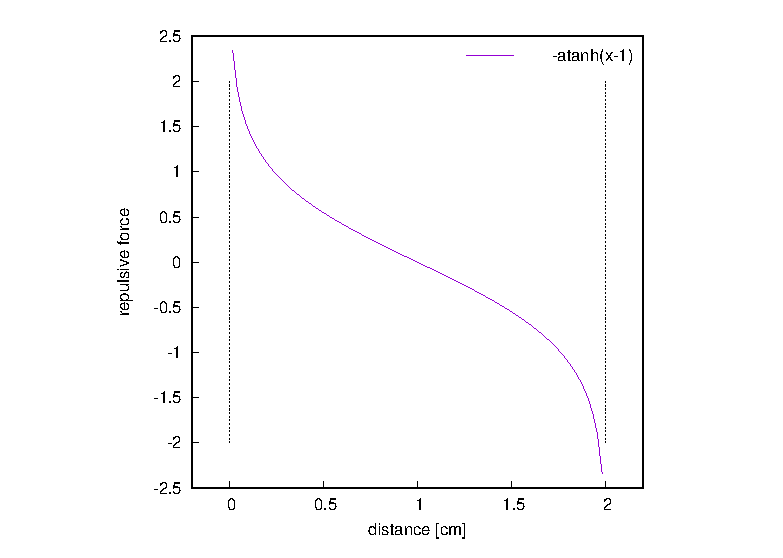
\includegraphics[width=1.0\hsize]{plot/minus_atanh.eps}
    \end{center}
    \caption{ほげほげ}
    \label{fig::atanh}
  \end{figure}

\subsection{画像認識}
  炎上ポールの認識には配布されたRapspberry Pi NoIR Camera V2(以下,カメラモジュール)を使用する.
  画像撮影から最も近い(と思われる)ポールへのベクトルを出力する一連の手順を,簡単に以下に示す.

  \begin{description}
    \item[画像取得] \mbox{} \\
      カメラモジュールへのアクセスには既成ライブラリ\cite{raspicam}を利用した.
      撮影によりピクセル値の二次元配列(cv::Mat)が出力として得られる.
      画像サイズの大小が及ぼす処理時間への影響は極めて大きいが,
      それが画像処理結果の精度に与える影響は未検証であるため,
      現在は適当な値が設定されている.\\
    \item[カラーモデル変換] \mbox{} \\
      得られた画像のカラーモデルをRGBからHSVに変更する.\\
    \item[2値画像化] \mbox{} \\
      HSV画像データに対し赤色マスクをかけて二値画像に変換する.
      赤色マスクの範囲は適当.\\
    \item[ノイズ除去] \mbox{} \\
      適当に膨張・縮小を繰り返してノイズを除去する.
      ちゃんとやってる処理じゃねえから現状ほとんど意味がねえ.\\
    \item[構造解析] \mbox{} \\
      2値画像中の輪郭線を検出した後,それを矩形で囲む.
      囲んだ矩形を縦横比で解析し,ポールの縦横比に対して$\pm 20 \%$以上の差があるものを除外する.
      残った矩形の重心点を求めて,適当にベクトルを作る.\\
  \end{description}

\begin{thebibliography}{9}
  \bibitem{raspicam} "RaspiCam: C++ API for using Raspberry camera with/without OpenCV",\\
                     "\texttt{https://www.uco.es/investiga/grupos/ava/node/40}",2017年5月31日最終確認.
\end{thebibliography}

\end{document}

  
\subsection{今後の予定}
図\ref{fig:schedule}に大まかな今後の予定を示す.
\begin{figure}[bH]
\begin{center}
  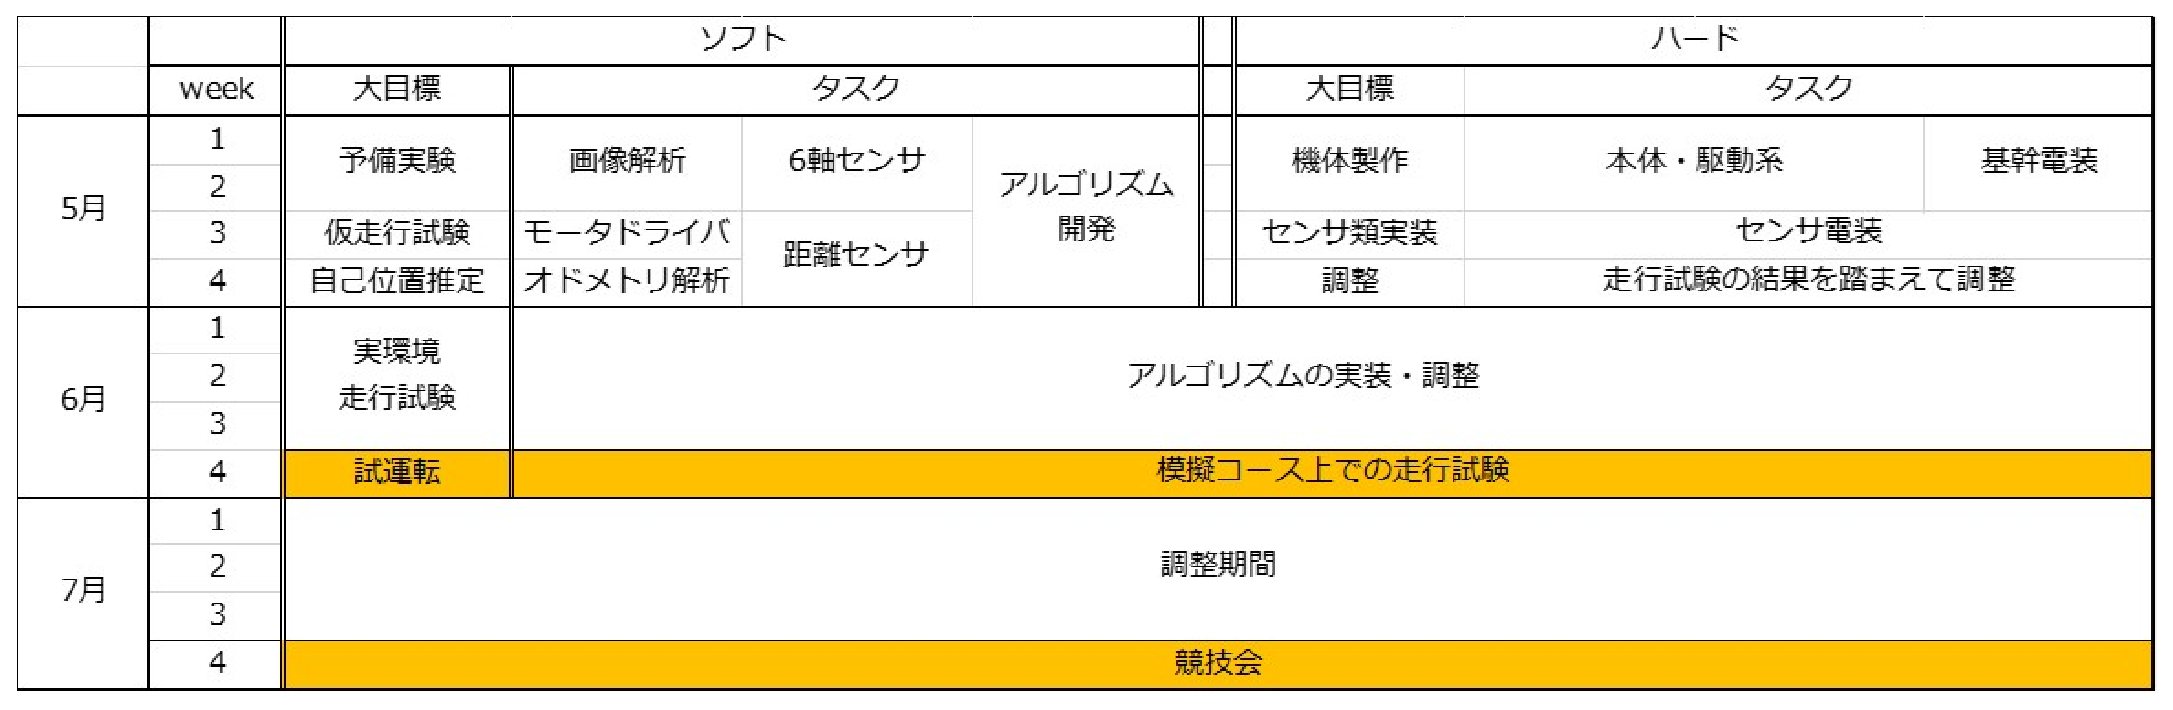
\includegraphics[width=1.0\hsize]{./picture/schedule.eps}
 \caption{今後の予定}
 \label{fig:schedule}
\end{center}
\end{figure}



\section{使用物品}
今回のRCRで使用する予定の物品を表\ref{tab:list1},\ref{tab:list2}に示す.5月31日時点での合計金額は79248円である.
\begin{table}[H]
 \begin{center}
  \caption{配布物品}
  \label{tab:list1}
  \begin{tabular}{|l|l|r|c|r|}  \hline
   メーカー & 商品名 & 単価 & 数量 & 価格 \\ \hline \hline 
   秋月電子通商 & ピンヘッダ(1X40) & 35円 & 1 & 35円  \\     \hline
   秋月電子通商 & ピンヘッダ(2X40) & 50円 & 1 & 50円  \\     \hline   
   秋月電子通商 & ソケット(2X40) & 95円 & 1 & 95円  \\     \hline
   秋月電子通商 & スミチューブ(黒) & 40円 & 1 & 40円 \\ \hline
   秋月電子通商 & スミチューブ(赤) & 40円 & 1 & 40円 \\ \hline
   秋月電子通商 & スミチューブ(クリア) & 40円 & 1 & 40円 \\ \hline
   秋月電子通商 & ハンダ & 280円 & 1 & 280円 \\ \hline
   秋月電子通商 & ハンダ吸い取り線 & 190円 & 1 & 190円 \\ \hline
   日本圧着端子 & XHベース 2極  & 10円 & 2 & 20円  \\     \hline
   日本圧着端子 & XHベース 3極  & 10円 & 7 & 70円  \\     \hline
   日本圧着端子 & XHベース 4極  & 10円 & 6 & 60円  \\     \hline
   日本圧着端子 & XHコネクタ 2極  & 10円 & 2 & 20円  \\     \hline
   日本圧着端子 & XHコネクタ 3極  & 10円 & 7 & 70円  \\     \hline
   日本圧着端子 & XHコネクタ 4極  & 10円 & 6 & 60円  \\     \hline
   日本圧着端子 & 圧着端子(XH)  & 4円 & 15 & 60円  \\     \hline
   &  & &合計 & 1130円  \\   \hline
  \end{tabular}
 \end{center}
\end{table}

\newpage

\begin{table}[H]
 \begin{center}
  \caption{引き継ぎ品}
  \label{tab:list1}
  \begin{tabular}{|l|l|r|c|r|}  \hline
   メーカー & 商品名 & 単価 & 数量 & 価格 \\ \hline \hline 
   TAMIYA & タミヤギヤードモータ & 4860円 & 2 & 9720円  \\     \hline
   TAMIYA & ギヤードモータハブシャフトセット & 540円 & 1 & 9720円   \\  \hline
   TAMIYA & ミディアムナローレーシンググラジアルタイヤ & 540円 & 1 & 540円  \\  \hline
   TAMIYA & ミディアムナロー5本スパークホイール & 540円 & 1 & 540円   \\     \hline
   TAMIYA & SP.106 7.2Vコネクタ & 270円 & 2 & 540円  \\      \hline
   RSコンポーネンツ株式会社 & カメラモジュール &  2740円 & 1 & 2740円  \\ \hline
   RSコンポーネンツ株式会社 & Rasberry Pi 3 ケース & 1080円 & 1 & 1080円  \\    \hline
   RSコンポーネンツ株式会社 & Raspberry Pi 3 Model B & 6200円 & 1 & 6200円  \\     \hline
   MISUMI & トグルスイッチ & 80円 & 2 & 160円 \\       \hline
   MISUMI & キャスターホイール & 990円 & 1 & 990円 \\     \hline
   KHK & 歯車(モジュール 0.5 歯数60) &1360円 & 4 & 5440円 \\      \hline
   KHK & プラスチックナット+連結スペーサーセット & 100円 & 1 & 100円  \\      \hline
   秋月電子通商 & 3軸加速度センサモジュール & 850円 & 1 & 850円  \\     \hline
   秋月電子通商 & 3軸ジャイロセンサモジュール & 750円  & 1 & 750円 \\     \hline
   Cytron &DCブラシモータドライバ & 2160円 & 2 & 4320円 \\       \hline
   Powers & POWER MAX 4000 Ni-MH& 4000円 & 2 & 8000円  \\     \hline
   シャープ株式会社 & シャープ測距モジュール & 400円 & 6 & 2400円  \\    \hline
   株式会社矢島製作所 & ユニバーサル基盤 & 100円 & 2 & 200円 \\    \hline
   日本電産コパル電子 & ロータリエンコーダ & 7500円 & 2 & 15000円  \\   \hline
   Arduino Srl & Arduino UNO & 3240円 & 1 & 3240円  \\     \hline
   TOSHIBA & microSDHC メモリーカード 8GB & 1058円 & 1 & 1058円  \\    \hline
   OptoSupply & スペーサー & 45円 & 4 & 180円  \\     \hline
   GWS &サーボモータ & 1000円 & 1 & 1000円  \\    \hline
   ルビコン株式会社 & 電解コンデンサ(47μF) & 10円 & 2 &20円 \\     \hline
   &  & &合計 & 65608円  \\   \hline
  \end{tabular}
 \end{center}
\end{table}

\newpage
\begin{table}[H]
 \begin{center}
  \caption{新規購入品}
  \label{tab:list2}
  \begin{tabular}{|l|l|l|r|c|r|}  \hline
   取引先 & 商品名 & 型番または商品コード & 単価 & 数量 & 価格 \\   \hline \hline
   Strawberry Linux & 近距離センサモジュール & VL6180X & 1296円 & 3 & 3888円 \\    \hline
   Strawberry Linux & 降圧型DC-DCコンバータ & LT8697 & 1404円 & 1 & 1404円  \\      \hline
   秋月電子通商 & シャープ測距モジュール & GP2Y0E03 & 760円 & 1 & 760円  \\      \hline
   秋月電子通商 & I2Cバス用双方向レベル変換モジュール & PCA9306 & 150円 & 1 & 150円  \\      \hline
   misumi & 15mm角アルミフレーム & KHFS3-15 & 673円 & 1 & 673円  \\      \hline
   misumi & 15mm角アルミフレーム用四角ナット & HNSQ3-3 & 600円 & 1 & 600円  \\       \hline
   misumi & 15mm角アルミフレーム用ブラケット & HBLTBS3 & 75円 & 20 & 1500円  \\      \hline
   misumi & 小径玉軸受 & FL686ZZ & 440円 & 4 & 1760円  \\      \hline
   misumi & イグリデュールG フランジ型軸受 & GFM-0608-25 & 75円 & 5 & 375円 \\     \hline
   misumi & アルミ 角パイプ & HFHQ1515-1.5-500 & 200円 & 1 & 200円  \\       \hline
   秋月電子通商 & モータドライバ & TA7291P & 300円 & 1 & 300円  \\      \hline
   横山テクノ & アルミ 丸パイプ 6×1.0×400 & & 310円 & 1 & 310円 \\        \hline
   ヨドバシカメラ & ミニモータ低速ギアボックス & 70189 & 716円 & 1 & 716円  \\      \hline
   & & & & 合計 & 11610円  \\      \hline
  \end{tabular}
 \end{center}
\end{table}




\begin{thebibliography}{9}
 \bibitem{raspicam}
    "RaspiCam: C++ API for using Raspberry camera with/without OpenCV",\\
    "\texttt{https://www.uco.es/investiga/grupos/ava/node/40}",\\
    2017年5月31日最終確認.

  \bibitem{elinux}
    "RPi Camera Module - eLinux.org",\\
    "\texttt{http://elinux.org/Rpi\_Camera\_Module\#Technical\_Parameters\_.28v.2\_board.29}",\\
    2017年5月31日最終確認.
\end{thebibliography}


\newpage
\setcounter{page}{1}
\pagestyle{fancy}
\renewcommand{\headrulewidth}{0.0pt}
\rhead{付録\thepage}
\lhead{}
\cfoot{}
\begin{verbatim}
  void setup() {
     Serial.begin(9600) ;
    }
    void loop() {
     int ans ;

     ans = analogRead(0)  ;
     Serial.println(ans) ;
     delay(500) ;
    }	
\end{verbatim}
    

\end{document}
